%%%%%%%%%%%%%%%%%%%%%%%%%%%%%%%%%%%%%%%%%
% Programming/Coding Assignment
% LaTeX Template
%
% This template has been downloaded from:
% http://www.latextemplates.com
%
% Original author:
% Ted Pavlic (http://www.tedpavlic.com)
%
% Note:
% The \lipsum[#] commands throughout this template generate dummy text
% to fill the template out. These commands should all be removed when 
% writing assignment content.
%
% This template uses a Perl script as an example snippet of code, most other
% languages are also usable. Configure them in the "CODE INCLUSION 
% CONFIGURATION" section.
%
%%%%%%%%%%%%%%%%%%%%%%%%%%%%%%%%%%%%%%%%%

%----------------------------------------------------------------------------------------
%	PACKAGES AND OTHER DOCUMENT CONFIGURATIONS
%----------------------------------------------------------------------------------------

\documentclass{article}

\usepackage[utf8]{inputenc}
\usepackage[italian]{babel} 
\usepackage{fancyhdr} % Required for custom headers
\usepackage{lastpage} % Required to determine the last page for the footer
\usepackage{extramarks} % Required for headers and footers
\usepackage[usenames,dvipsnames]{color} % Required for custom colors
\usepackage{graphicx} % Required to insert images
\usepackage{listings} % Required for insertion of code
\usepackage{courier} % Required for the courier font
\usepackage{lipsum} % Used for inserting dummy 'Lorem ipsum' text into the template
\usepackage{mathtools}
\DeclarePairedDelimiter{\ceil}{\lceil}{\rceil}
\DeclarePairedDelimiter\floor{\lfloor}{\rfloor}

% Margins
\topmargin=-0.45in
\evensidemargin=0in
\oddsidemargin=0in
\textwidth=6.5in
\textheight=9.0in
\headsep=0.25in

\linespread{1.1} % Line spacing

% Set up the header and footer
\pagestyle{fancy}
\lhead{\hmwktitolobreve} % Top left header
\lfoot{\lastxmark} % Bottom left footer
\cfoot{} % Bottom center footer
\rfoot{Page\ \thepage\ of\ \protect\pageref{LastPage}} % Bottom right footer
\renewcommand\headrulewidth{0.4pt} % Size of the header rule
\renewcommand\footrulewidth{0.4pt} % Size of the footer rule

\setlength\parindent{0pt} % Removes all indentation from paragraphs

%----------------------------------------------------------------------------------------
%	CODE INCLUSION CONFIGURATION
%----------------------------------------------------------------------------------------

\definecolor{MyDarkGreen}{rgb}{0.0,0.4,0.0} % This is the color used for comments
\lstloadlanguages{Perl} % Load Perl syntax for listings, for a list of other languages supported see: ftp://ftp.tex.ac.uk/tex-archive/macros/latex/contrib/listings/listings.pdf
\lstset{language=Perl, % Use Perl in this example
        frame=single, % Single frame around code
        basicstyle=\small\ttfamily, % Use small true type font
        keywordstyle=[1]\color{Blue}\bf, % Perl functions bold and blue
        keywordstyle=[2]\color{Purple}, % Perl function arguments purple
        keywordstyle=[3]\color{Blue}\underbar, % Custom functions underlined and blue
        identifierstyle=, % Nothing special about identifiers                                         
        commentstyle=\usefont{T1}{pcr}{m}{sl}\color{MyDarkGreen}\small, % Comments small dark green courier font
        stringstyle=\color{Purple}, % Strings are purple
        showstringspaces=false, % Don't put marks in string spaces
        tabsize=5, % 5 spaces per tab
        %
        % Put standard Perl functions not included in the default language here
        morekeywords={rand},
        %
        % Put Perl function parameters here
        morekeywords=[2]{on, off, interp},
        %
        % Put user defined functions here
        morekeywords=[3]{test},
       	%
        morecomment=[l][\color{Blue}]{...}, % Line continuation (...) like blue comment
        numbers=left, % Line numbers on left
        firstnumber=1, % Line numbers start with line 1
        numberstyle=\tiny\color{Blue}, % Line numbers are blue and small
        stepnumber=5 % Line numbers go in steps of 5
}

% Creates a new command to include a perl script, the first parameter is the filename of the script (without .pl), the second parameter is the caption
\newcommand{\perlscript}[2]{
\begin{itemize}
\item[]\lstinputlisting[caption=#2,label=#1]{#1.pl}
\end{itemize}
}


%----------------------------------------------------------------------------------------
%	NAME AND CLASS SECTION
%----------------------------------------------------------------------------------------


\newcommand{\hmwkDueDate}{\date{\today}} % Due date
\newcommand{\hmwkClass}{Tecniche di Preprocessing in C++ applicate a problemi lineari misto-interi (MIP) } % Course/class
\newcommand{\hmwktitolobreve}{MIP Preprocessing} %
\newcommand{\hmwkUniversita}{Università degli Studi Di Milano} % Teacher/lecturer
\newcommand{\hmwkAuthorName}{Marco Odore} % Your name

%----------------------------------------------------------------------------------------
%	TITLE PAGE
%----------------------------------------------------------------------------------------

\title{
\vspace{2in}
\textmd{\textbf{\hmwkClass}}\\
\vspace{0.1in}\large{\textit{\hmwkUniversita}}
\vspace{3in}
}

\author{\textbf{\hmwkAuthorName}}
\date{\today} % Insert date here if you want it to appear below your name

%----------------------------------------------------------------------------------------

\begin{document}

\maketitle

%----------------------------------------------------------------------------------------
%	TABLE OF CONTENTS
%----------------------------------------------------------------------------------------

%\setcounter{tocdepth}{1} % Uncomment this line if you don't want subsections listed in the ToC

\newpage
\tableofcontents
\newpage

%----------------------------------------------------------------------------------------
%	PROBLEM 1
%----------------------------------------------------------------------------------------

% To have just one problem per page, simply put a \clearpage after each problem

\section{Scopo del lavoro}

Il lavoro propone una possibile implementazione in C++ di alcune delle tecniche di preprocessing applicate ai problemi di ottimizzazione lineare misto-interi (MIP) e binary (BIP). Per validare la correttezza del software è stato realizzato un generatore randomico di problemi MIP/BIP da sottomettere poi in AMPL. 

\subsection{Tecniche implementate}

Sono state implementate diverse tecniche adatte a diversi contesti della programmazione lineare:

\begin{itemize}
\item Riduzione dei bound sulle variabili (Bounds Tightening)
\item Ricerca di vincoli non soddisfacibili (Detecting Infeasibility)
\item Eliminazione di vincoli ridondanti (Detecting Redundant Constraints)
\item Fissaggio delle variabili (Variables Fixing)
\item Riduzione dei coefficienti nei problemi BIP (Coefficients Reduction)
\end{itemize}

\section{Bounds Tightening}

La riduzione dei bound è una tecnica applicabile a tutti i tipi di variabili, e cioè a quelle di tipo continuo, intero e binario.
\newline
\newline
Questo metodo di preprocessing consiste nell'iterare sui vincoli del problema verificando la presenza di bound migliori per ogni variabile esaminata. Il procedimento continua finché, una volta iterati tutti i vincoli, ci sono stati degli aggiornamenti sui bound.
\newline
\newline
Procedimento:
\begin{itemize}
\item Per ogni vincolo si considerano separatamente le variabili con coefficienti positivi da quelle con coefficienti negativi:
\[
\sum_{a_{ij}>0}a_{ij} x_{j} + \sum_{a_{ij}<0}a_{ij} x_{j} \le b_i  \;\;\;\forall i
\] 
\item Si isola una variabile k alla volta, cercando di ottimizzare i suoi bound:
\[
a_{ik} x_{k} + \sum_{a_{ij}>0}a_{ij} x_{j} + \sum_{a_{ij}<0}a_{ij} x_{j} \le b_i
\]
\item Si passa poi al calcolo del possibile nuovo bound, che nel caso di variabile con coefficiente positivo sarà il nuovo upperbound $u'_k$, mentre nel caso di variabile con coefficiente negativo sarà il nuovo lowerbound $l'_k$:

\[
if\;\;a_{ij}>0:\]
\[
u'_k = \frac{1}{a_{ik}}\left(b_i - \sum_{j\ne k,a_{ij}>0}a_{ij} x_{j} + \sum_{a_{ij}<0}a_{ij} x_{j}\right)
\]

\[
if\;\;a_{ij}<0:\]
\[
l'_k = \frac{1}{a_{ik}}\left(b_i - \sum_{a_{ij}>0}a_{ij} x_{j} + \sum_{j\ne k,a_{ij}<0}a_{ij} x_{j}\right)
\]
\item Dopo i calcoli, i bound vengono effettivamente aggiornati, ponendo $u_k = u'_k$ o $l_k=l'_k$ se e solo se $u'_k<u_k$ o $l'_k>l_k$.
\end{itemize}

Nel caso le variabili siano intere (o binarie) viene semplicemente fatto il ceiling nel caso di nuovi lower bound ($\ceil*{l'_k}$) e floor nel caso di nuovi upper bound ($\floor*{u'_k}$).
\section{Detecting Infeasibility and Variables Fixing}
Per verificare se un vincolo è non soddisfacibile va calcolato prima di tutto il suo \textit{lower bound} $L_i$, che va poi confrontato con il termine noto $b_i$:

\[
L_i = \sum_{a_{ij}>0}a_{ij} l_{x_{j}} + \sum_{a_{ij}<0}a_{ij} u_{x_{j}}
\]

Se $L_i>b_i$, allora il vincolo risulta chiaramente insoddisfacibile e non esiste quindi una soluzione.
\newline
Se invece $L_i=b_i$, si possono fissare le variabili seguendo questo criterio:

\[\forall a_{ij}>0 \;\;\;\;\;\;\;\;\;\;\;\forall a_{ij}<0 \]
\[x_j = l_{x_{j}} \;\;\;\;\;\;\;\;\;\;\;\; x_j = u_{x_{j}}\]

\section{Detecting Redundant Constraints}
Per individuare vincoli ridondanti viene calcolato l'\textit{upper bound} $U_i$ del vincolo che si sta controllando, che poi viene confrontato con il suo termine noto $b_i$:

\[
U_i = \sum_{a_{ij}>0}a_{ij} u_{x_{j}} + \sum_{a_{ij}<0}a_{ij} l_{x_{j}}
\]

Se $U_i \le b_i $ allora il vincolo viene rispettato sempre, qualunque sia il valore assunto dalle variabili, e quindi può essere eliminato. 

\section{Coefficients Reduction}

Questa tecnica può essere applicata solo a problemi di programmazione lineare binaria (BIP). Consiste nel ridurre la grandezza dei coefficienti dei vincoli eseguendo una serie di operazioni.
\newline
\newline
Procedimento:

\begin{itemize}
\item Si considera un vincolo alla volta:
\[\sum_{a_{ij}>0}a_{ij}x_{j} + \sum_{a_{ij}<0}a_{ij}x_{j} \le b_i \]
\item Si ottiene il valore $M$ pari alla somma dei coefficienti positivi del vincolo $i$:
\[M = \sum_{a_{ij}>0}a_{ij} \]

\item Viene poi creato un set $S$ di coefficienti tali che il loro valore assoluto è maggiore di $M-b_i$:

\[
S=\{a_{ij}:|a_{ij}>M-b_i\}
\]
\item Se il set S non è vuoto seleziona un coefficiente $a_k$ al suo interno, e se $a_k>0$:

\[a'_k = M - b_i \]
\[b'_i = M - a_k \]
\[a_k = a'_k\]
\[b_i = b'_i\]

\item mentre se $a_k<0$:
\[ a'_k = b_i - M \]
\[ a_k = a'_k \]

Il procedimento viene iterato sul singolo vincolo finché il set $S$ ha almeno un elemento al suo interno.

\end{itemize}

\section{Preprocessing in C++}

Le tecniche citate sono state implementate in c++ sfruttando la programmazione a oggetti, cercando di realizzare un'astrazione dei tipi di variabili presenti all'interno dei problemi di programmazione MIP (continue, intere e binarie), in maniera tale da garantirne le proprietà intrinseche. 
\newline
\newline
\subsection{Le classi}
Praticamente è stata realizzata una classe astratta principale, chiamata \emph{Variable}, da cui derivano poi tutte le altre tipologie di variabili/classi, e cioè le classi \textit{intVar} e \textit{floatVar}. La variabile binaria è stata rappresentata da una classe derivata di \textit{intVar} chiamata \textit{binVar}, essendo un caso particolare di variabile intera.
\newline
\newline
L'\textit{overriding} dei metodi di queste classi, in particolare \textit{setMin} e \textit{setMax}, ha permesso di garantire le proprietà intrinseche delle variabili (vincoli sui bound, sul tipo di dato).
\newline
\newline
Nella Figura \ref{UML} è mostrato lo schema UML che mostra la struttura gerarchica delle classi utilizzate per rappresentare le variabili.
\newline
\newline
Per quanto riguarda invece la rappresentazione dei coefficienti e dei termini noti è stata realizzata una semplice matrice di dimensione $i \times n$, dove $i$ è il numero di vincoli del problema, e $n$ è il numero delle variabili sommato ad 1, che rappresenta il termine noto. Un esempio di matrice è rappresentata nella Figura \ref{matrix}.
\begin{figure}[ht]
\centering
\[
10x_1 + 3x_2 + 5x_3 - 6x_4 \le 7
\]
\[
-2x_1 + 2x_3 +3x_4 \le -1
\]
\[
\left[\begin{matrix}10 & 3 & 5 & -6 & 7 \\ -2 & 0 & 2 & 3 & -1\end{matrix}\right]
\]
\caption{\footnotesize{La matrice dei coefficienti + termini noti ottenuta dall'insieme di vincoli dell'esempio.}}
\label{matrix}
\end{figure}
\begin{center}
\begin{figure}
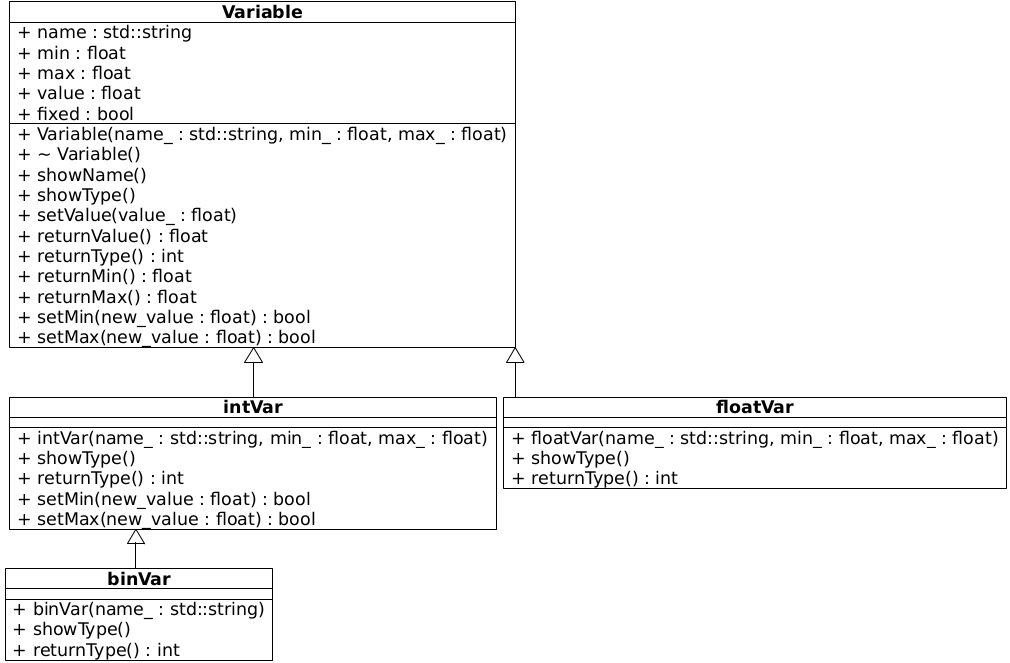
\includegraphics[scale=0.38]{uml.png}
\caption{\footnotesize{Lo schema UML delle classi che rapprentano le variabili in c++-}}
\label{UML}
\end{figure}
\end{center}
\subsection{Le funzioni}
Per quanto riguarda le funzioni scritte per le tecniche di preprocessing, sono state implementate:

\begin{itemize}
\item La funzione \textit{boundsPreprocess} che prova a restringere i bound sulle variabili.
\item La funzione \textit{constraintsPreprocess} che verifica la presenza di vincoli
non soddisfacibili, di vincoli ridondanti e di variabili che è possibile fissare.
\item La funzione \textit{coefficientsReduction}, applicabile solo al caso binario, che si occupa di provare la riduzione sui coefficienti.
\end{itemize}

Oltre a queste sono state implementate altre funzioni di utilità, come funzioni di stampa a console dell'insieme di vincoli e variabili (\textit{printConstraints}), e funzioni di scrittura su file di tipo \textit{.dat} (\textit{writeDat}), che sono file utilizzabili in AMPL, un linguaggio di programmazione matematica.

\section{Validazione del lavoro}
Per verificare la correttezza del lavoro si è sfruttato AMPL, un linguaggio di programmazione matematica.
%----------------------------------------------------------------------------------------

\end{document}